%%%%%%%%%%%%%%%%%%%%%%%%%%%%%%%%%%%%%%%%%%%%%%%%%%%%%%%%%%%%%%%%%%%%%%%%%%


% abnTeX2: Modelo de Trabalho Acadêmico em conformidade com 
% as normas da ABNT


%%%%%%%%%%%%%%%%%%%%%%%%%%%%%%%%%%%%%%%%%%%%%%%%%%%%%%%%%%%%%%%%%%%%%%%%%%


\documentclass[english, 
               brazil, 
               bsc] %Opções bsc (TCC) e msc (Mestrado)
               {dcomp-abntex2}




%%%%%%%%%%%%%%%%%%%%%%%%%%%%%%%%%%%%%%%%%%%%%%%%%%%%%%%%%%%%%%%%%%%%%%%%%%
% Área para adição de pacotes extras
%%%%%%%%%%%%%%%%%%%%%%%%%%%%%%%%%%%%%%%%%%%%%%%%%%%%%%%%%%%%%%%%%%%%%%%%%%


\usepackage{float}
\usepackage{pgfgantt}
\usepackage{lscape}



\restylefloat{table}


%Utilize aqui seu pacote preferido para algoritmos
\usepackage[linesnumbered]{algorithm2e}


%%%%%%%%%%%%%%%%%%%%%%%%%%%%%%%%%%%%%%%%%%%%%%%%%%%%%%%%%%%%%%%%%%%%%%%%%%


%Compila o índice
\makeindex


\begin{document}


% Seleciona o idioma do documento (conforme pacotes do babel)
\selectlanguage{brazil}


% Retira espaço extra obsoleto entre as frases.
\frenchspacing 


%%%%%%%%%%%%%%%%%%%%%%%%%%%%%%%%%%%%%%%%%%%%%%%%%%%%%%%%%%%%%%%%%%%%%%%%%%
% ELEMENTOS PRÉ-TEXTUAIS
%%%%%%%%%%%%%%%%%%%%%%%%%%%%%%%%%%%%%%%%%%%%%%%%%%%%%%%%%%%%%%%%%%%%%%%%%%


\pretextual




\titulo{PreOCR - Trabalho de Processamento de Imagens T01 2023.2} 
\autor{Grupo 13 - Everton Santos de Andrade Júnior}
\orientador{}
\coorientador{}


% \inserirInformacoesPDF





% \inserirInformacoesPDF
%
%
\imprimircapa
% \imprimirfolhaderosto*
%  
%     
\mostrarSUMARIO


%%%%%%%%%%%%%%%%%%%%%%%%%%%%%%%%%%%%%%%%%%%%%%%%%%%%%%%%%%%%%%%%%%%%%%%%%%
% ELEMENTOS TEXTUAIS
%%%%%%%%%%%%%%%%%%%%%%%%%%%%%%%%%%%%%%%%%%%%%%%%%%%%%%%%%%%%%%%%%%%%%%%%%%


\textual


%%%%%%%%%%%%%%%%%%%%%%%%%%%%%%%%%%%%%%%%%%%%%%%%%%%%%%%%%%%%%%%%%%%%%%%%%%
% Introdução
%%%%%%%%%%%%%%%%%%%%%%%%%%%%%%%%%%%%%%%%%%%%%%%%%%%%%%%%%%%%%%%%%%%%%%%%%%
\chapter{Introdução e Resultados} \label{introduction}

Neste trabalho, desenvolvemos um programa capaz de processar imagens binárias no formato PBM ASCII (PGM tipo P1), contendo texto dos tipos e tamanhos de fontes, variando de 8 à 40. Conseguimos determinar o básico do trabalho que são o número de linhas e palavras no texto e os retangulos dessas palavras, gerando uma imagem de saída com esses retangulos. Além disso, nosso grupo implementou mais funcionalidades, como a detecção de colunas e blocos (ou paragrafos) do texto, utilizando o conceito de distância alinhada, includindo a \textit{bouding box} (bbox) desses blocos e linhas que indicam as colunas. Também foi feito a detecção dos das bbox dos caracteres quer formam as palavras encontradas. Aprós isso é feito uma ánalise de similaridades entre as imagem de letras padrões e as letras encontradas nessa detecção através template matching \cite[12.2]{gonzalez2008digital}. O template matching não gerou bons reconhecimentos, mesmo após testar diferentes variações como desconderar a igualdade de pixels pretos ou brancos.

Adicionalmente, para ilustrar nossos resultados de forma mais interativa, geramos uma série de imagens intermediárias que mostram o processo de detecção de blocos, colunas, palavras, e linhas destacando as regiões por um retangulo de diferentes cores. O formato dessas imagems é P3 (ascii RGB). Essas imagens foram usadas em sequencia de frames para gerar um video de saída auxiliando na depuração e compreensão do comportamento do algoritmo usando o programa de linha de commando ``ffmpeg``.

O processamento envolve filtro mediano e, principalmente, dialtação. Também envolve os conceitos de connectividade para encontrar as palavras. A nossa abordagem é dinamica, baseado na altura das palavras mudamos os parametros enquanto o programa roda. Desse modo é possivel identificar estruturas de texto em diferentes alinhamentos, como justificado, esquerda, centro e direita, além de lidar com diferentes tamanhos e estilos de fonte, incluindo Comic Sans, Impact, Cascadia Code, Arial e Times New Roman. Um exemplo de video gerado pode ser encontrado em \url{https://youtu.be/uA45GeodGss?si=ZOgsA2av7EKZeG69}.

Decidimos começar brevemente com os resultados (\autoref{ch-resultados}). Em seguida no \autoref{ch-notas} com intruções e notas sobre o projeto o qual inclui os passoes necessários para execução e as definição das imagem teste de entrada. No \autoref{ch-detalhes}, damos detalhes sobre os algoritmos implementados. Por fim, o \autoref{ch-conclusão} discute sobre possiveis melhorias e palavras finais de conclusão.


\chapter{Resultados} \label{ch-resultados}
 Os resultados desse projeto podem ser bem entendidos pelas imagens coloridas geradas, por isso, os próximos parafos discutem a saída gerada por este projeto para diferentes entradas. Na \autoref{cascadia} temos o resultado gerado no projeto para a entrada de um texto na fonte Cascadia Code em negrito de tamanho 10, alinhado à esquerda. Essa imagem tem baixa resolução e vem com ruídos. Mesmo assim o nosso trabalho conseguiu identificar as bbxoes das palavras, mesmo quando as letras possuvem alturas diferentes. Os retangulos em vermelho indicam essas bboxes das palavras encontradas. A linha em amarelo é feita pelo algortimo todas vez que encontra o começo de  uma coluna. Em verde está o agrupamento dos blocos ou paragrafos que o nosso trabalho conseguiu encontrar. Especificamente para essa entrada, o algoritmo encontrou 5 blocos, 2 colunas, 42 linhas e 395 palavras. Com a mesma fonte mas de tamanha 16, e centralizado, temos outro resultado na \autoref{cascadia16}, nesse encontramos 2 colunas, 4 blocos, 38 linhas e 226 palavras.

Na \autoref{timesnewroman}, ja mudamos a fonte para Time News Roman, e ainda está em itálico. Nesse entrada já pulamos para quartro colunas e tamanho 18 de fonte. No resultado foi encontrado 4 colunas, 6 blocos, 38 linhas e 197 palavras. O correto deveria ser 196 palavras, o restante está correto. Pulamos para uma nova fonte chamada Impact de tamanho 40, que é um grande salto dos outros casos. Neste, o algortimo encontra 2 colunas, 2 blocos, 18 linhas e palavras 47 palavras. O correto deveria ser 46 palavras, o restante está correto.

Ademais, foram realizados teste com fonte Arial, com exemplos tanto providos pela professor Beatriz, quanto criados pelo grupo. Um exemplo desses resultados pode ser ilutrado pela \autoref{arial}, nesse o texto é justificado com 3 colunas e tamanho 12. O algortimo encontrou tudo corretamente, com 557 palavras e 52 linhas.  A \autoref{comi} inclue o resultado para um exemplo com letras de tamanho 8 e fonte Comic Sans, a menor testada no projeto. Por fim, demos upload da coleção de videos gerados por este trabalho com  diferentes fontes e tamanhos testados que pode ser encontrado no youtube neste link: \url{https://www.youtube.com/watch?v=uA45GeodGss}.

Também houve a detecção de caracteres, os resultados te encontrar o retangulos dos caracteres numa dada palavra funciona perfeitamente, até onde pudemos testar, pois letras são conectadas, então basta utilizar a mesma função de conectividade usada pra encontrar as palavras, mas sem fazer dilatação das imagens, pois não queremos juntas as letrar e sim manter-as separadas. A \autoref{chars} mostra um exemplo de bboxes encontrada para as letras num palava encontrada.


\begin{figure}[htb]
        \caption{\label{char} \small Exemplos de caracteres detectados para as palavras nesse, tremenedo e volta. }
        \begin{center}
            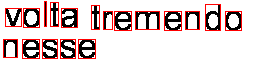
\includegraphics[scale=0.55]{./images/ocr.png}
        \end{center}
  \legend{ \small Fonte: Autor.}
\end{figure}


\begin{figure}[H]
        \caption{\label{cascadia} \small Cacadia Code em negrito, com 10 de tamanho, 2 colunas e 5 blocos de texto. A entrada possue baixa resolução e ruídos. }
        \begin{center}
            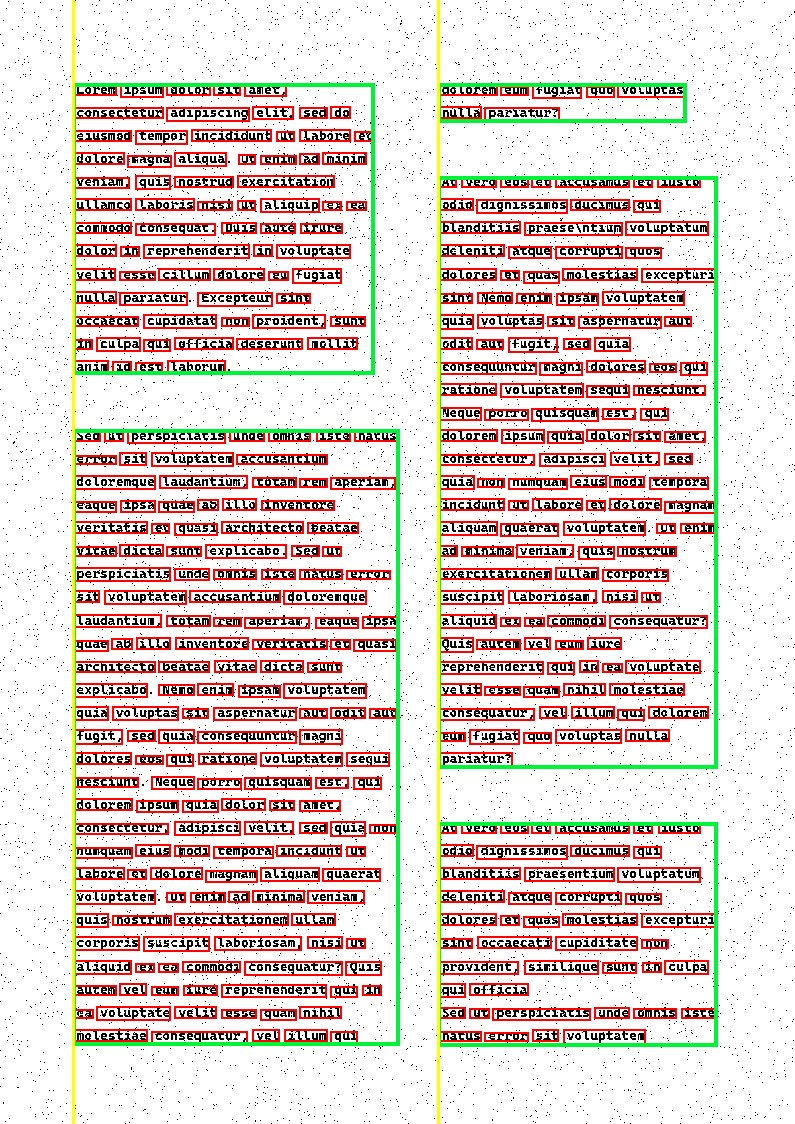
\includegraphics[scale=0.55]{./images/cascadia_code_10_detected_colunas_2_blocos_5_linhas_42_palavras_395.png}
        \end{center}
  \legend{ \small Fonte: Autor.}
\end{figure}

\begin{figure}[H]
        \caption{\label{cascadia16} \small Cacadia Code centralizado, com 16 de tamanho, 2 colunas e 4 blocos de texto. }
        \begin{center}
            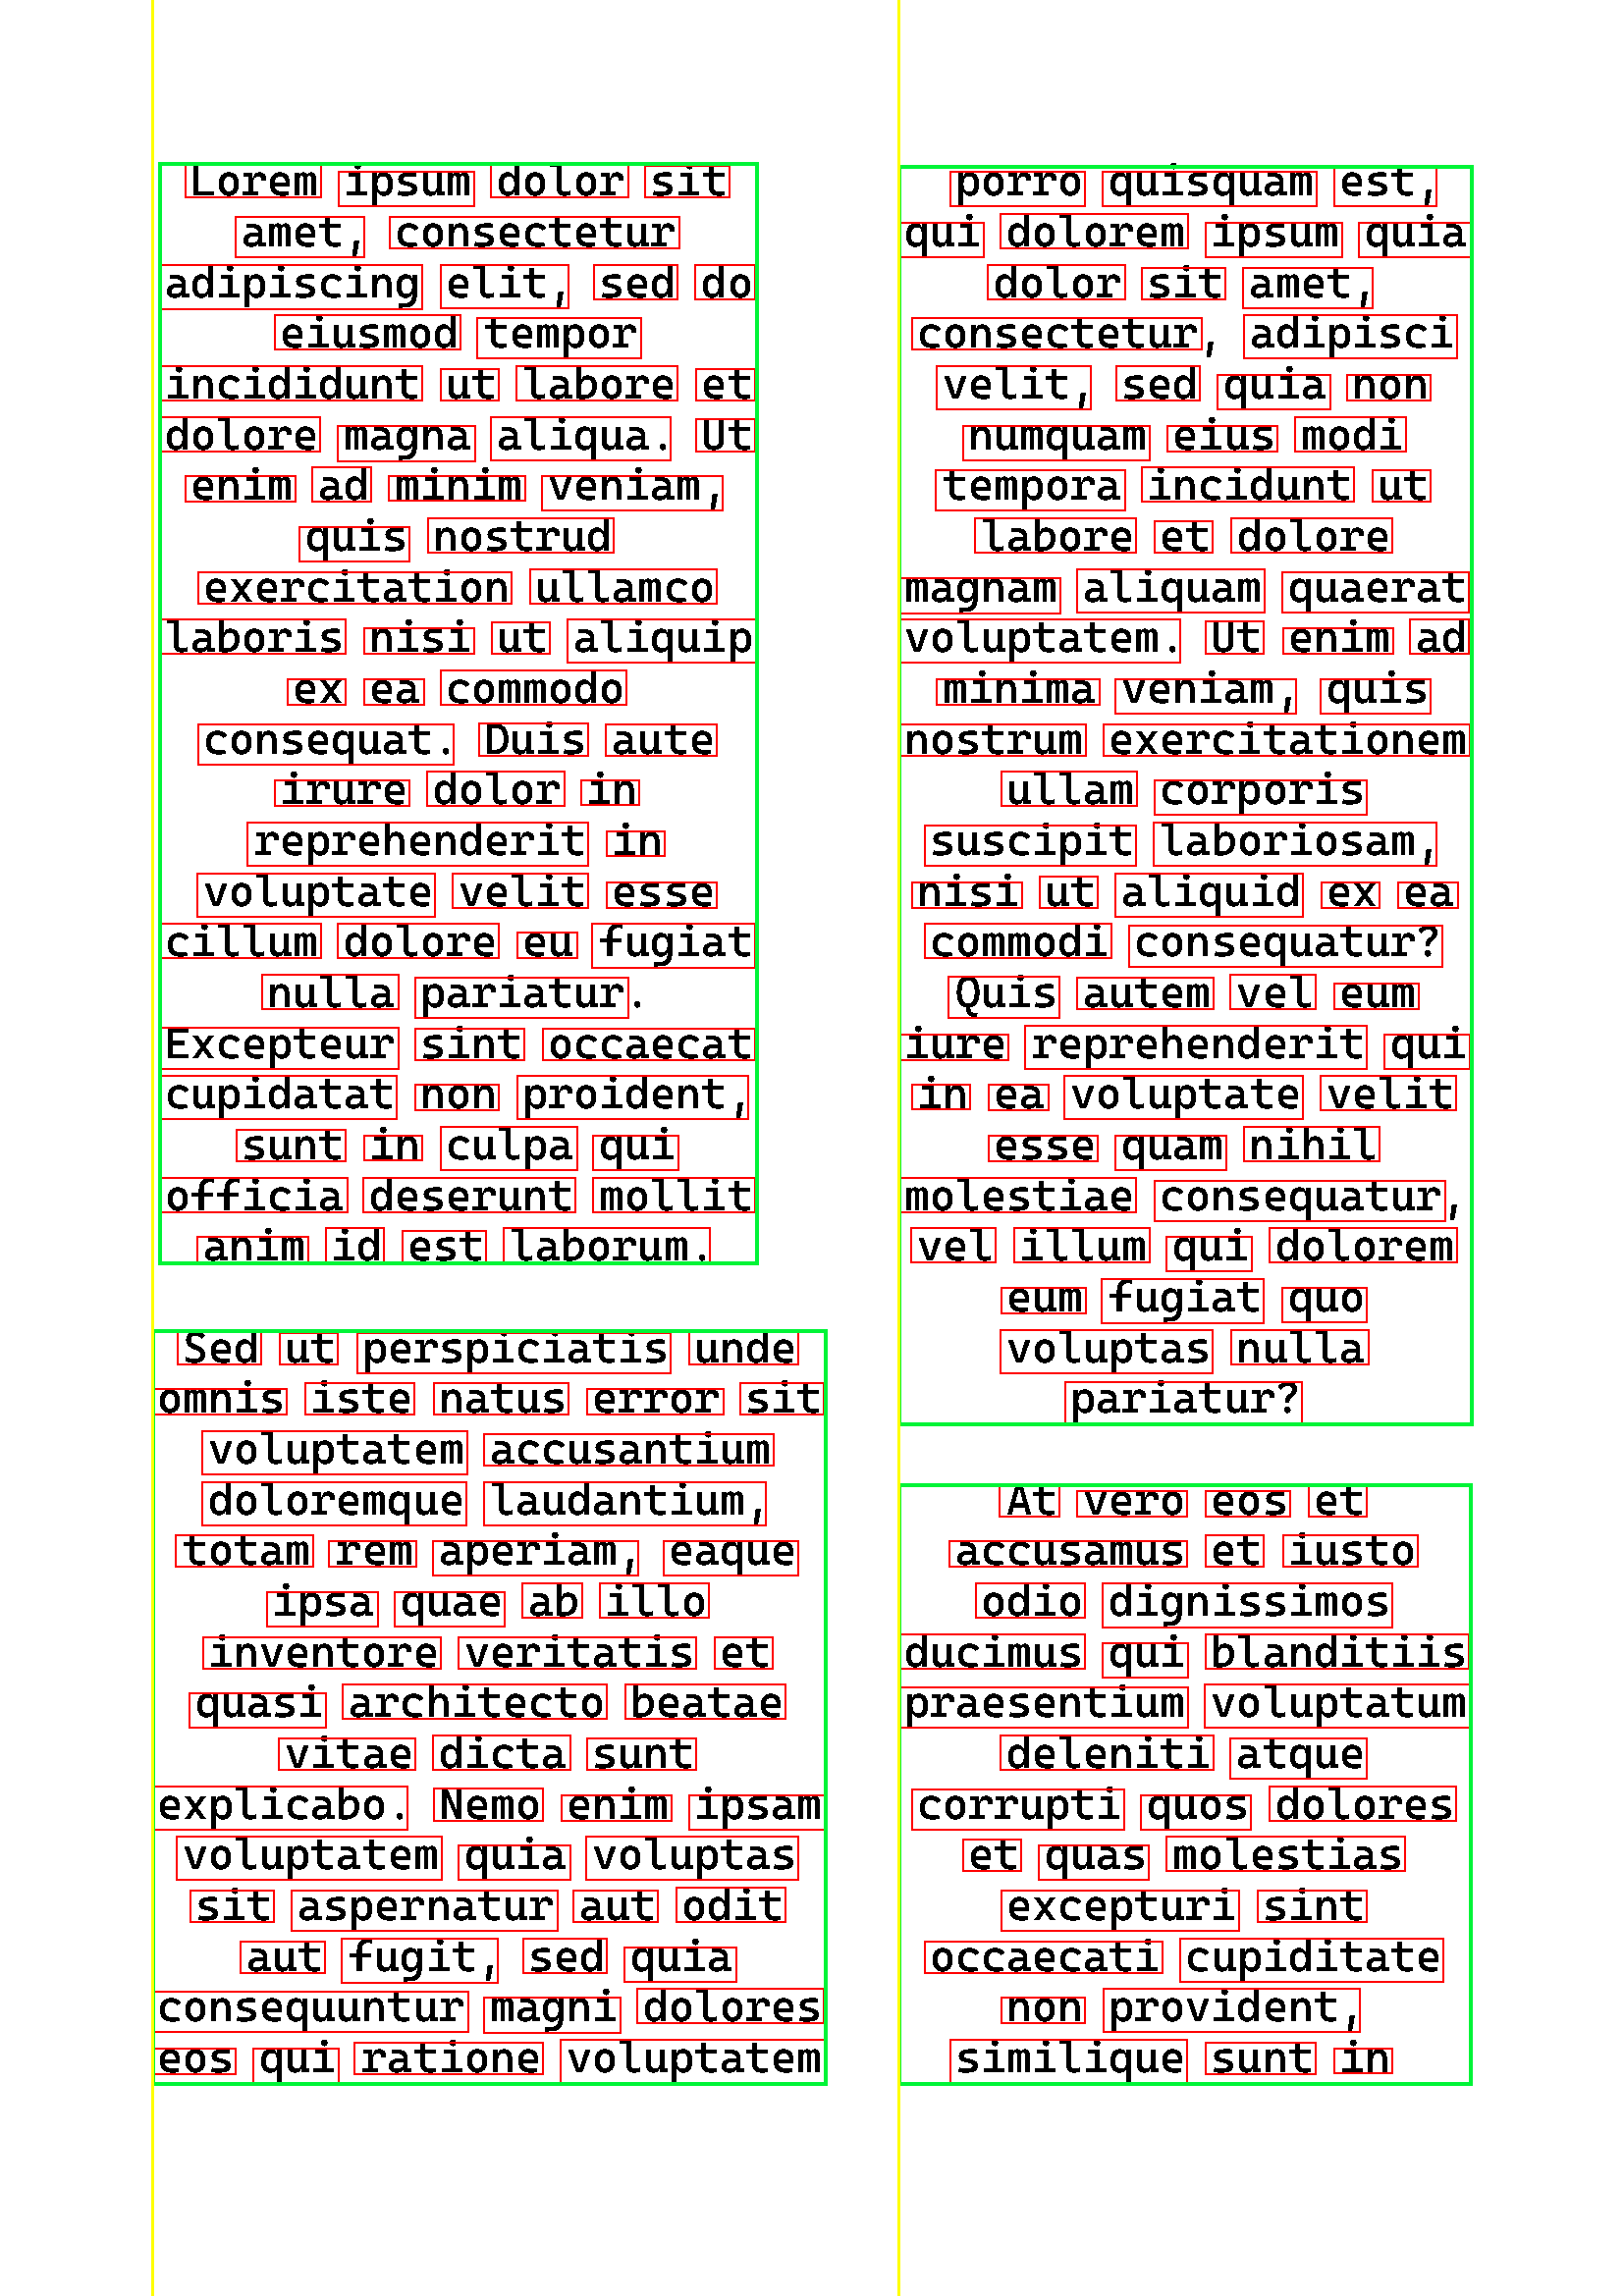
\includegraphics[scale=0.25]{./images/cascadia_code_centralizado_tamanho_16_colunas_2_blocos_4_linhas_38_palavras_226.png}
        \end{center}
  \legend{ \small Fonte: Autor.}
\end{figure}

\begin{figure}[H]
        \caption{\label{timesnewroman} \small Times News Roman em itálico, com 18 de tamanho, com 4 colunas, 6 blocos de texto.}
        \begin{center}
        \end{center}
        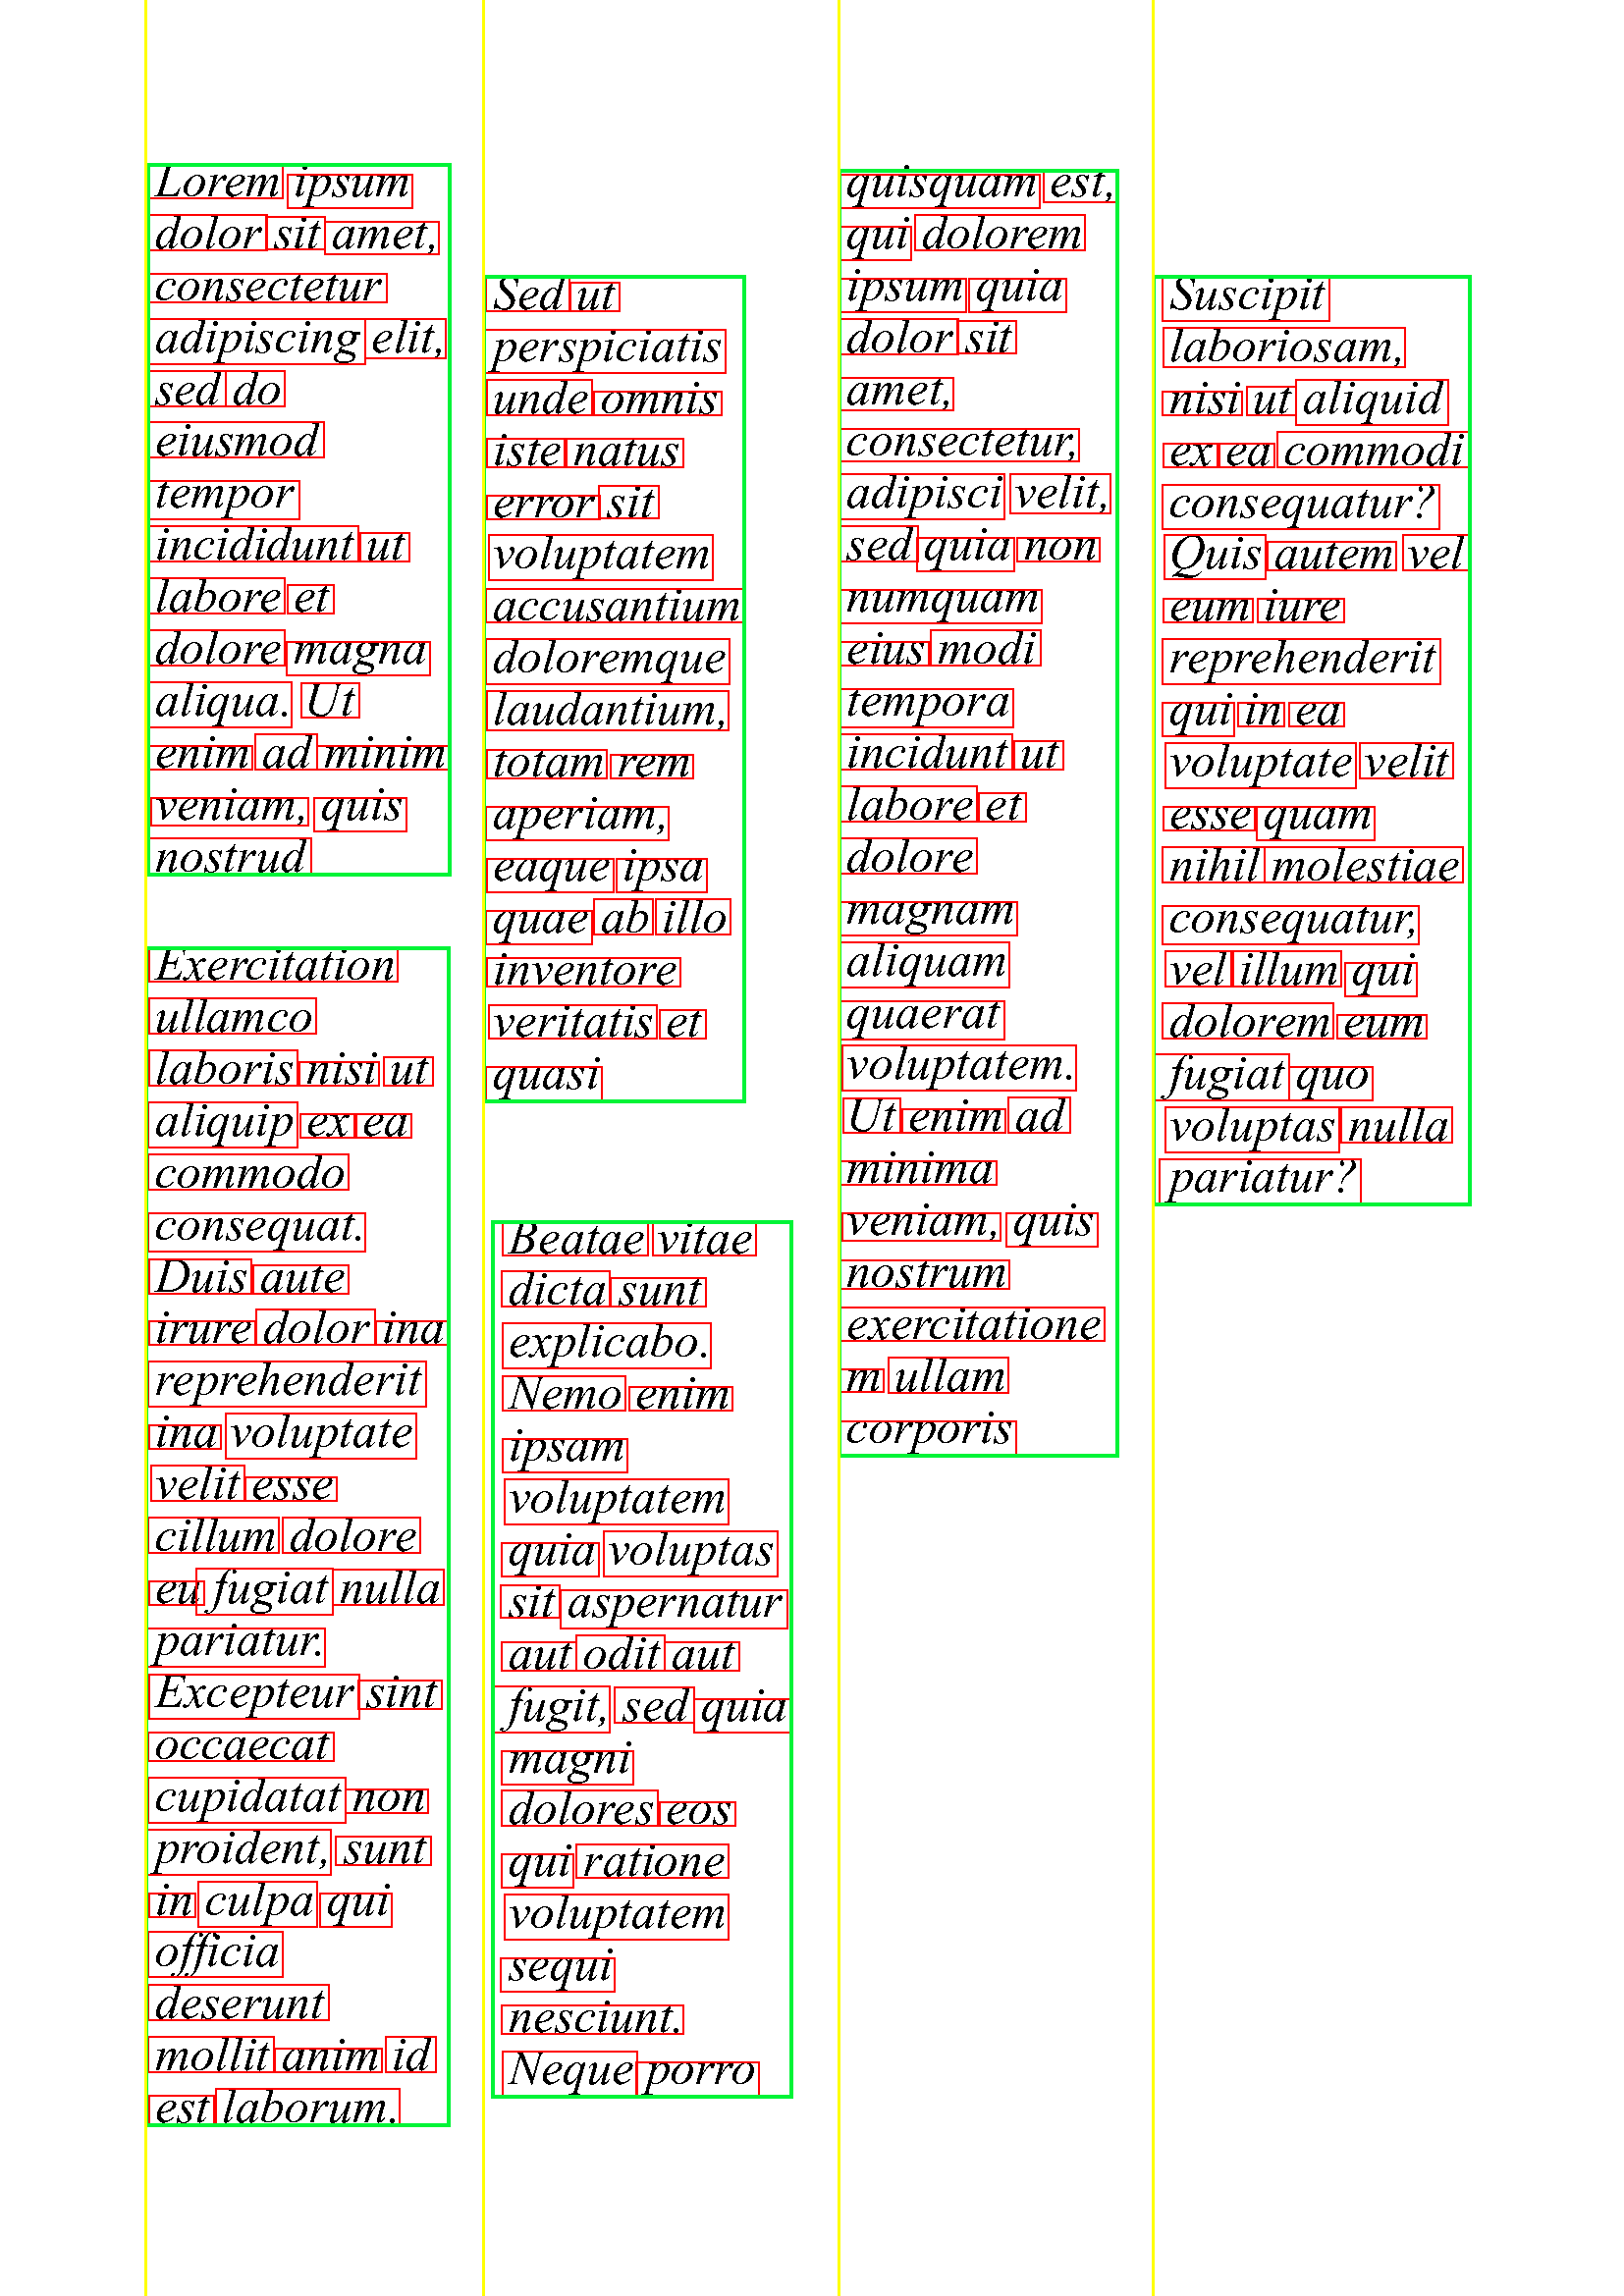
\includegraphics[scale=0.29]{./images/times_new_roman_colunas_4_blocos_6_linhas_38_palavras_197.png}
  \legend{ \small Fonte: Autor.}
\end{figure}


\begin{figure}[H]
  % impact_esquerda_tamanho_40_colunas_2_blocos_2_linhas_18_palavras_46
        \caption{\label{impact} \small Impact com tamanho 40, 2 colunas e 2 blocos de texto. }
        \begin{center}
            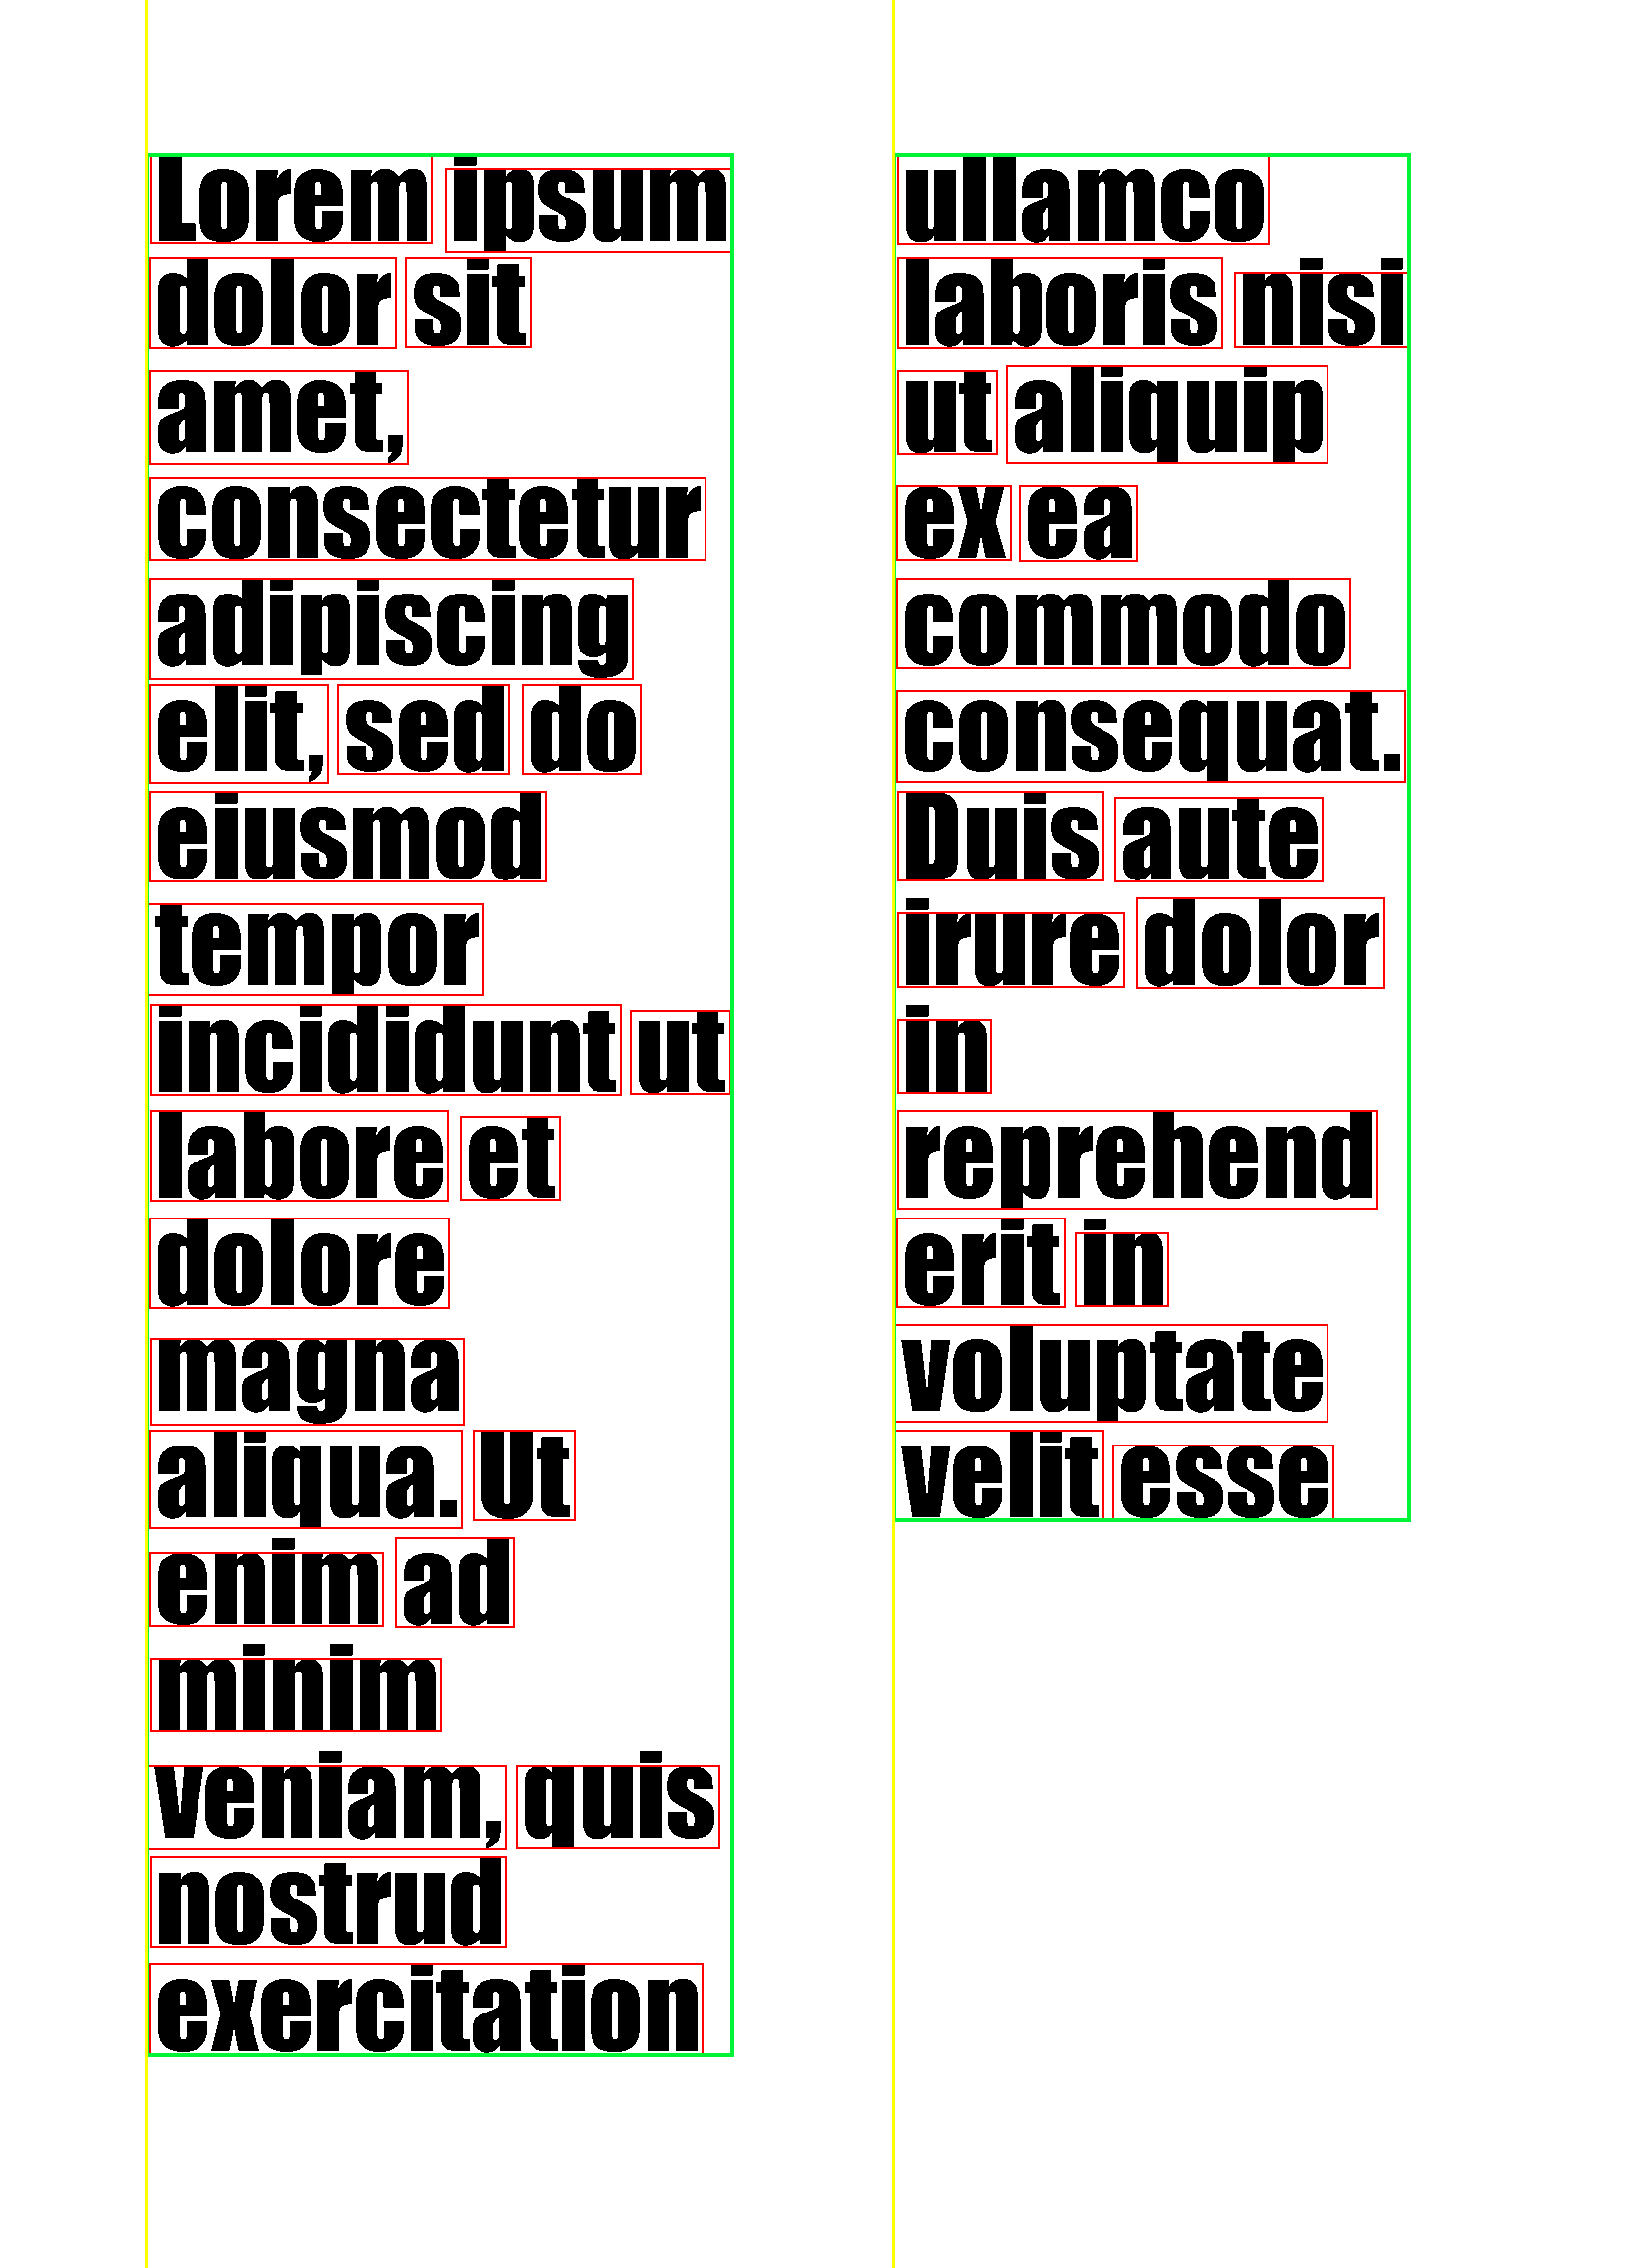
\includegraphics[scale=0.21]{./images/impact_columns.png}
        \end{center}
  \legend{ \small Fonte: Autor.}
\end{figure}

\begin{figure}[H]
        \caption{\label{comic} \small Comic Sans centralizado, com 8 de tamanho, 2 colunas e 5 blocos de texto.}
        \begin{center}
            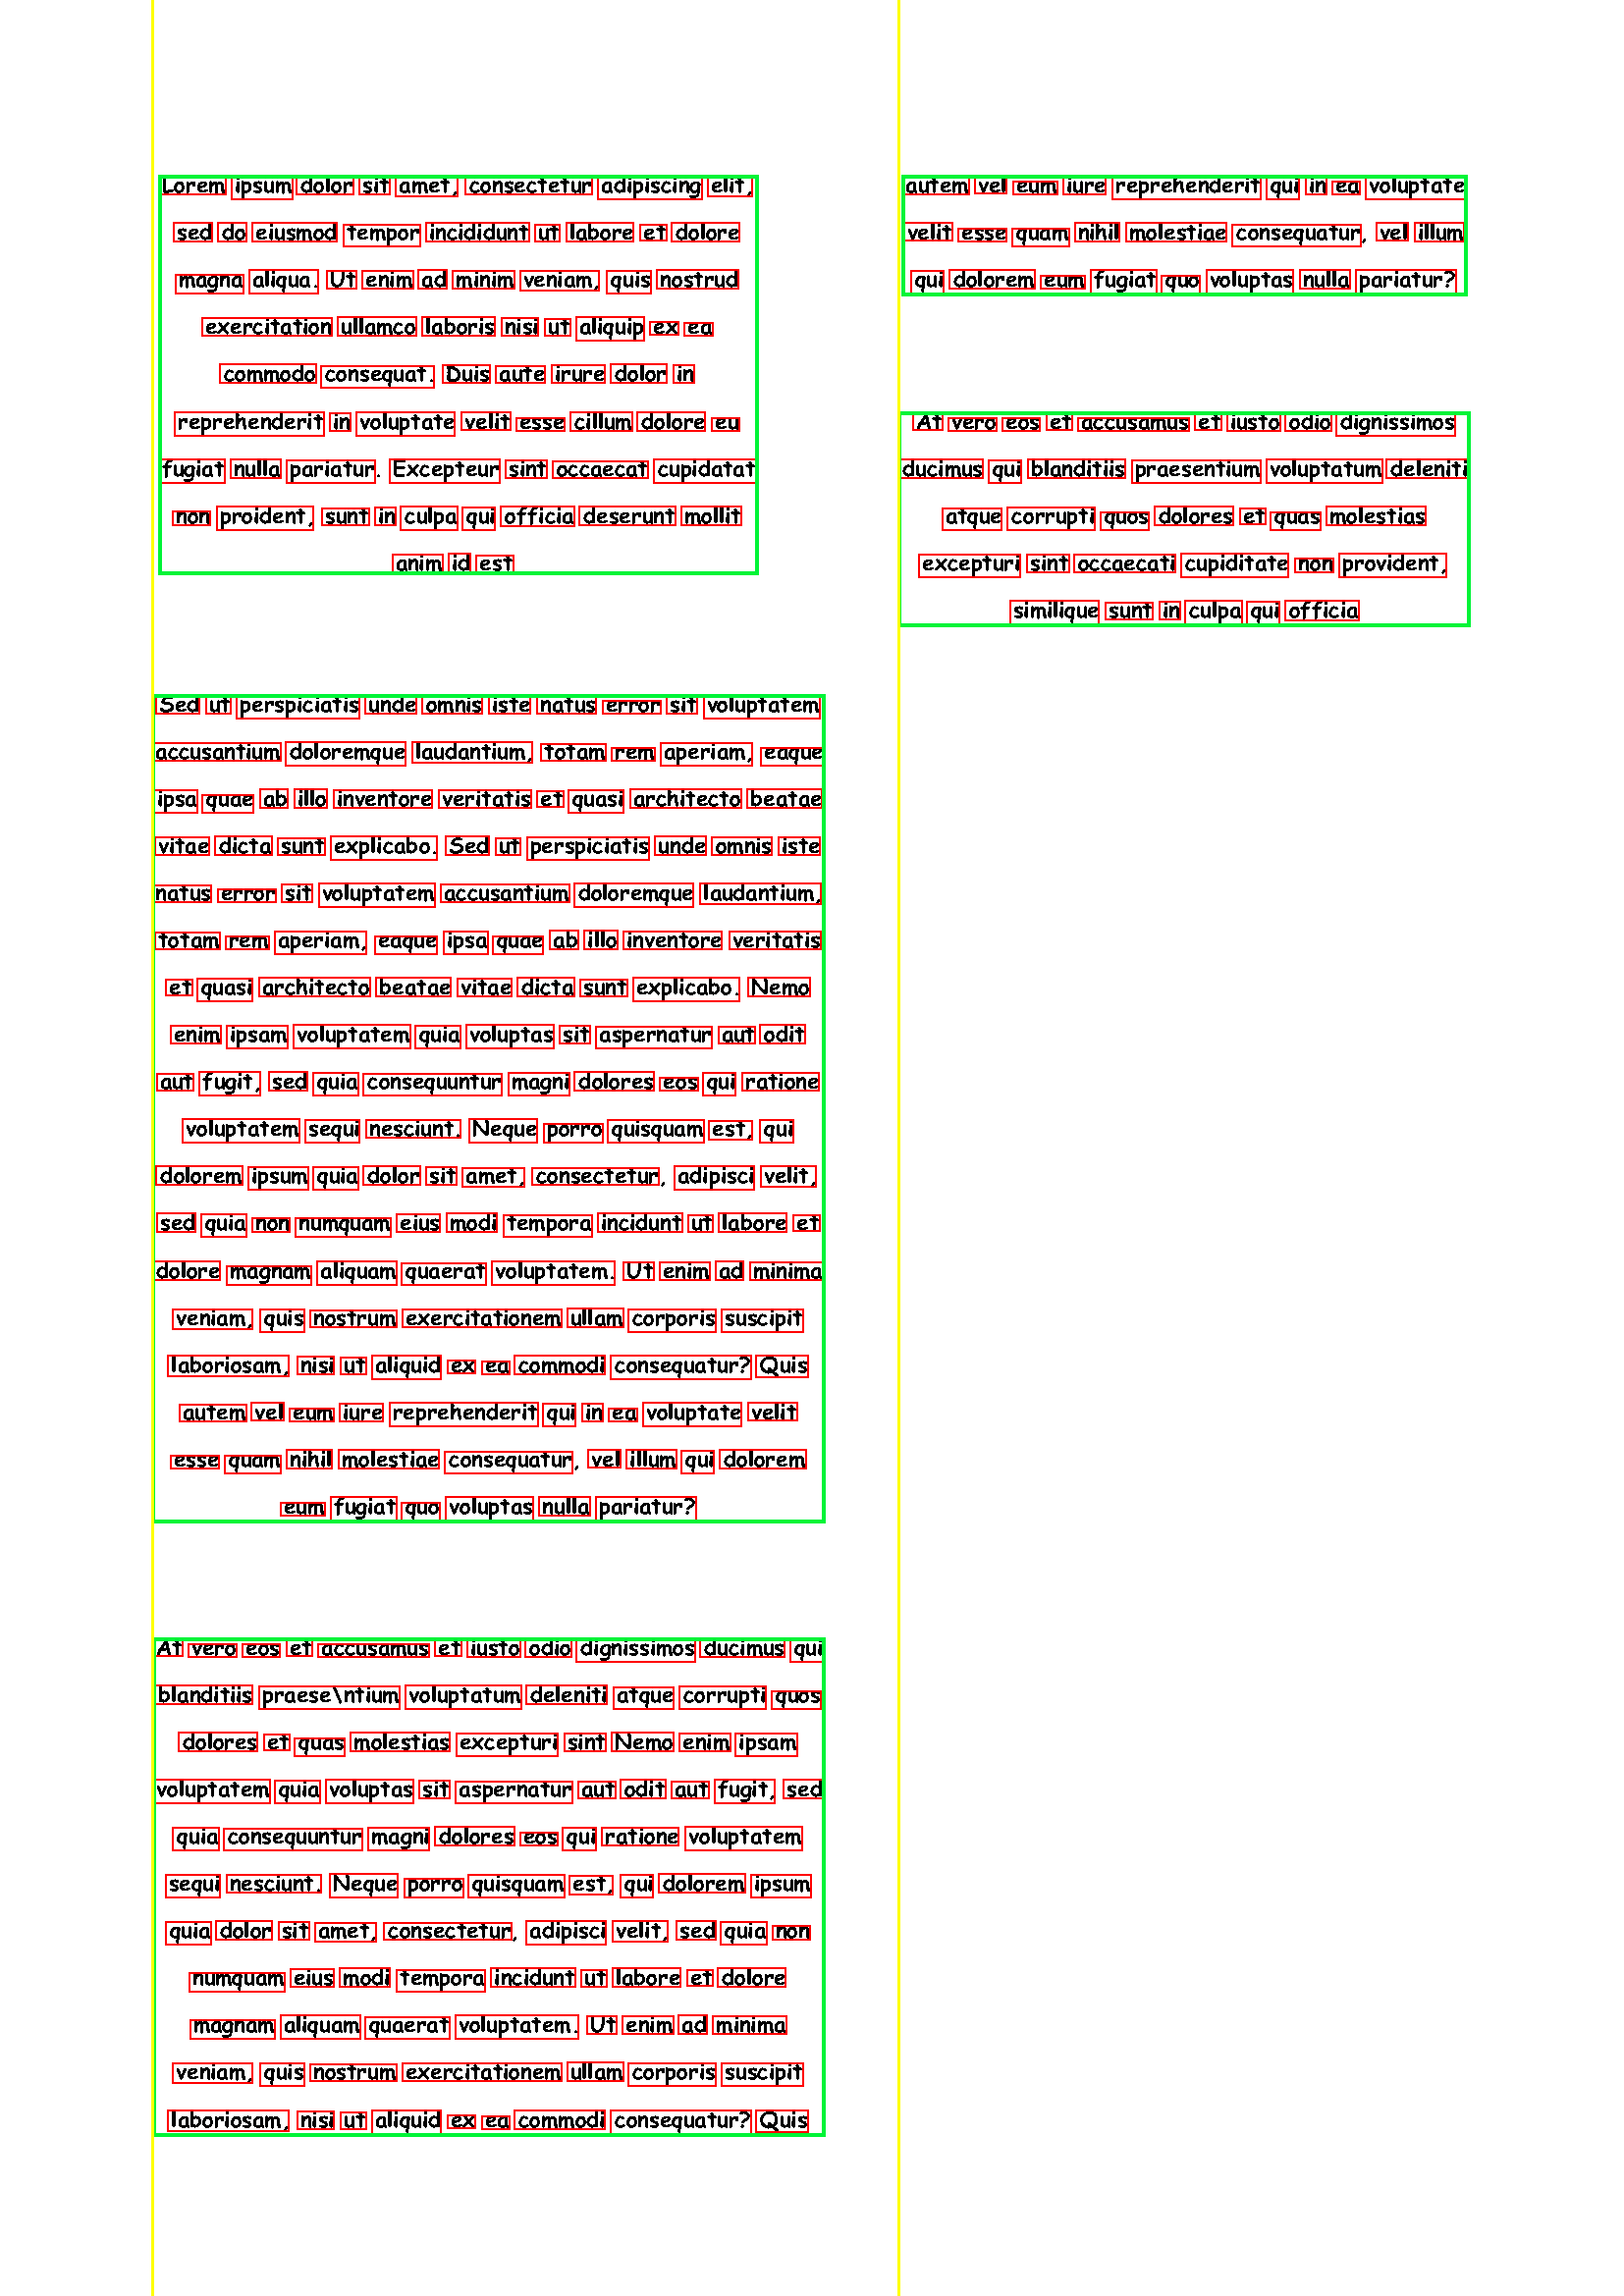
\includegraphics[scale=0.25]{./images/comic_sans_ms_bold_centralizado_tamanho_8_colunas_2_blocos_5_linhas_39_palavras_384.png}
        \end{center}
  \legend{ \small Fonte: Autor.}
\end{figure}

\begin{figure}[H]
        \caption{\label{arial} \small Arial justificado, com 12 de tamanho, 3 colunas e 8 blocos de texto.}
        \begin{center}
            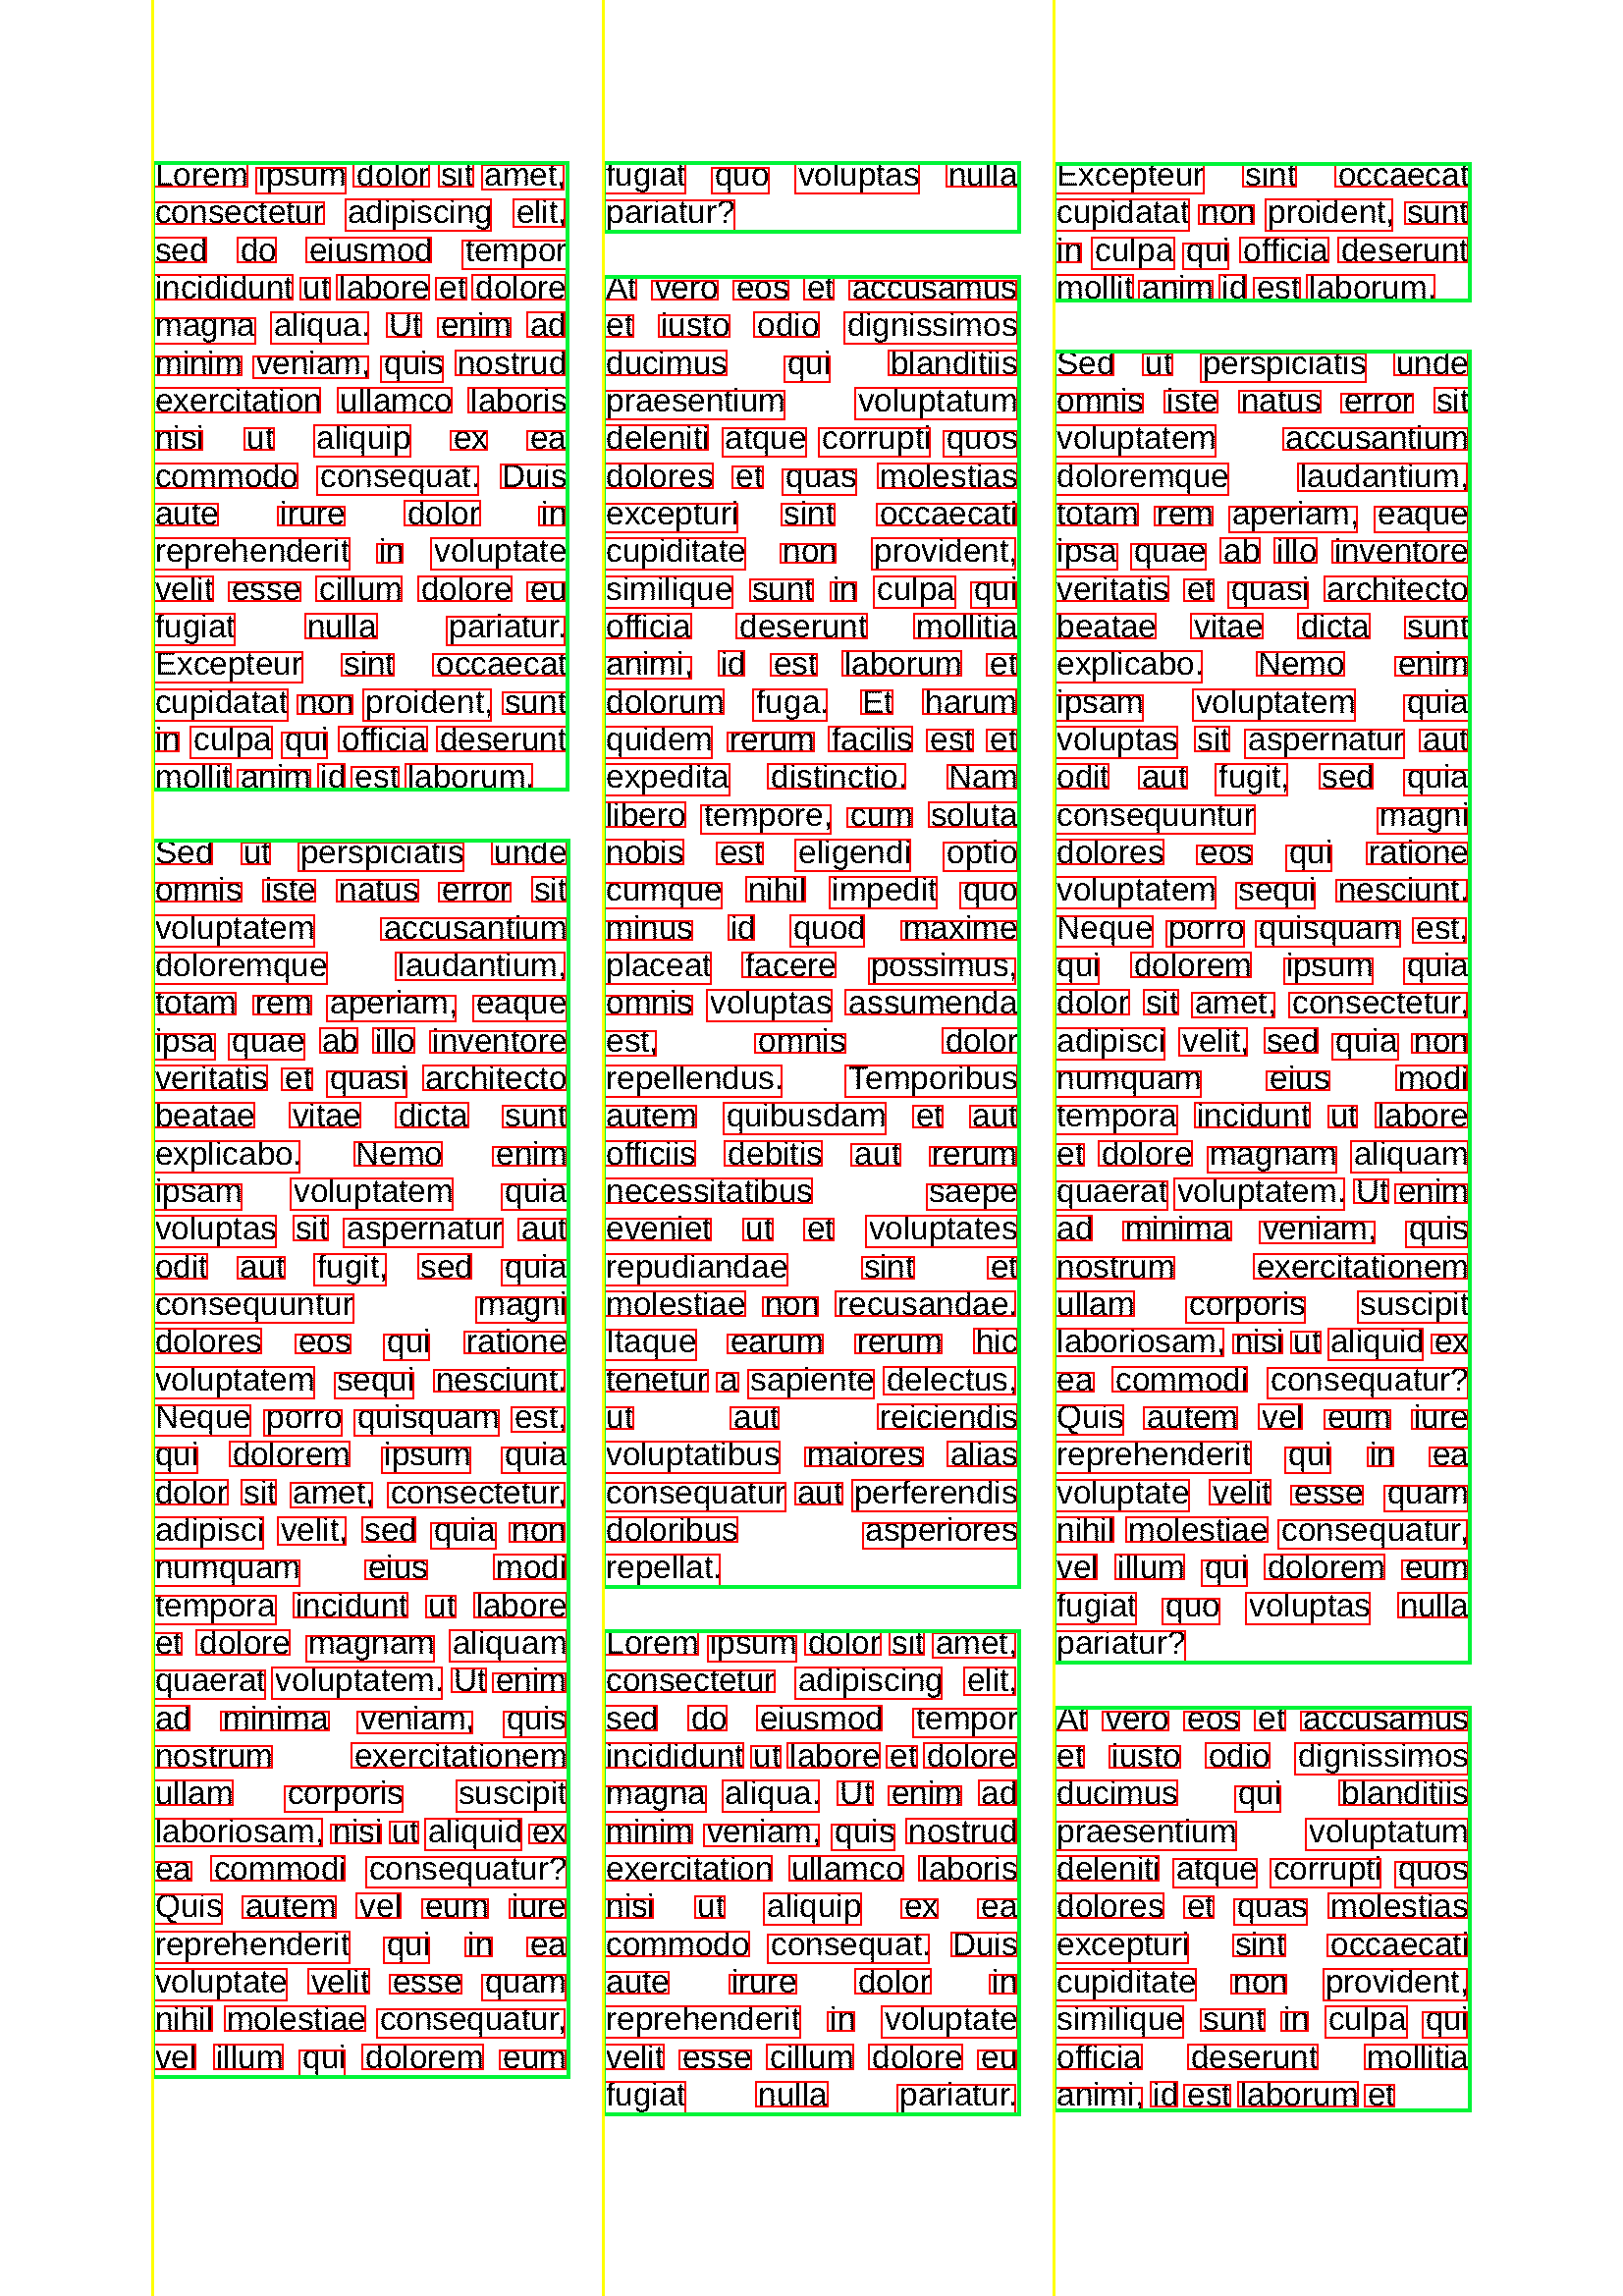
\includegraphics[scale=0.25]{./images/arial_justificado_tamanho_12_colunas_3_blocos_8_linhas_52_palavras_557.png}
        \end{center}
  \legend{ \small Fonte: Autor.}
\end{figure}


\chapter{Instruções \& Observações sobre o Projeto}
\label{ch-notas}

O repositório do projeto pode ser encontrado através do link \url{https://github.com/evertonse/pim}. O método proposto está implementado em Python e pode ser executado a partir da pasta raiz do projeto. Primeiro, certifique-se de ter o repositório do projeto clonado ou baixado. Em seguida, na linha de comando, navegue até a pasta raiz do projeto e execute o seguinte comando, substituindo \texttt{caminho/para/imagem.pbm} pelo caminho da imagem que deseja processar:

\begin{verbatim}
$ python3 src/main.py caminho/para/imagem.pbm
\end{verbatim}

Exemplo de caminho imagem pode ser:
\begin{verbatim}
python3 src/main.py assets/grupo_13_arial_esquerda_tamanho_16_colunas_2_blocos_4_linhas_39_palavras_318.pbm
\end{verbatim}

Se nenhuma imagem for fornecida, será usada uma imagem padrão. Imagens de exemplo adicionais geradas pelo nosso grupo podem ser encontradas na pasta "\texttt{assets}". Essas imagens seguem o padrão adaptado do documento PreOCR, pois precisamos identificar mais detalhes sobre a imagem. Seja $F$, $T$, $C$, $B$, $L$ e $P$ variáveis que representam informações sobre a fonte (tipo) e se é justificado, centralizado, etc., tamanho, número de colunas, número de linhas, número de blocos e número de palavras, respectivamente. Assim, o nome das imagens de teste segue o padrão \texttt{grupo\_13\_F\_tamanho\_T\_colunas\_C\_blocos\_B\_linhas\_L\_palavras\_P}. Um exemplo é:

\begin{itemize}
  \item \texttt{\small grupo\_13\_arial\_esquerda\_tamanho\_16\_
    colunas\_2\_blocos\_4\_linhas\_39\_palavras\_318}.
\end{itemize}

\section{Requisitos}
\begin{itemize}
  \item É necessário ter o Python instalado para executar o script. A versão testada foi 3.10 e 3.11, mas possivelmente pega em versões superiores à 3.4
  \item Opcionalmente se a ferramenta \texttt{ffmpeg} for instalada e esteja disponível no caminho do sistema o projeto irá gerar vídeos. No Ubuntu, \texttt{ffmpeg} pode ser instalado usando \texttt{sudo apt install ffmpeg} ou \texttt{sudo snap install ffmpeg}.
  \item A biblioteca \texttt{numpy} é necessária para manipulação eficiente das matrizes (listas de pythons são absurdamente lentas). Foi instalado apenas pela estutura de dados. As operações usadas do numpy são bem simples:  multiplicação de matriz por escalar; tirar o maximo ou minimo de matrizes; soma e subtração de matrizes. Pode ser instalada via \texttt{pip install numpy}. Se o \texttt{pip} não estiver instalado, ele pode ser obtido executando \texttt{sudo apt install python3-pip} no Ubuntu. \end{itemize}

\section{Observações}


Todos os arquivos gerados durante a execução do projeto são armazenados na pasta "\texttt{output/}", com exceção do arquivo principal que contém os retângulos das palavras em vermelho e do arquivo de vídeo. Esses dois arquivos são prefixados com "\texttt{group\_13}" e estão localizados no diretório atual.
O site \href{https://convertio.co/pdf-pbm/}{convertio.co} foi usado para converter arquivos PDF para o formato PBM para arquivos de entrada adicionais. As pastas e seus conteúdos, ilustrados na \autoref{folders}, estão organizados da seguinte forma:

\begin{itemize}
\item \textbf{src/}: diretório que contém o código-fonte do projeto.
\item \textbf{src/kernels.py}: definição dos elementos estruturante.
\item \textbf{src/main.py}: arquivo principal do projeto contendo o código de execução principal.
\item \textbf{src/ocr.py}: implementação da detectção e da tentativa de reconhecimento óptico de caracteres.
\item \textbf{src/pim.py}: implementação das funções de processamento de imagens usadas: dilatação, erosão, filtro mediana.
\item \textbf{src/utils.py}: contém funções de utilidade como ler imagem, escrever imagem, fazer resize de imagem.
\item \textbf{assets/}: contém as imagem \texttt{.pbm} criados pelo grupo.
\item \textbf{assets/letters/}: contém os modelos de letras utilizados na tentativa de reconhecimento de caracteres.
\item \textbf{assets/professora/}: contém as imagem .pbm disponibilizados pela professora, mas com os nomes adaptados.
\item \textbf{output/}: local onde são armazenados os arquivos gerados durante a execução do projeto, sendo apenas os resultados intermediários.
\end{itemize}

\begin{figure}[htb]
\caption{\small Estrutura de pastas do projeto.}
\label{folders}
    \begin{center}
    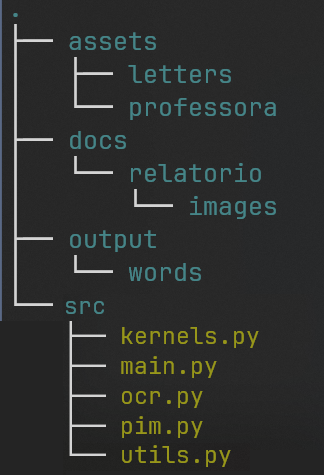
\includegraphics[scale=0.65]{./images/folders.png}
    \end{center}
\legend{ \small Fonte: Autor.}
\end{figure}

No exemplo de execução do projeto apresentado no \autoref{usage}, são fornecidas diversas informações úteis durante a execução do comando. Essas informações incluem o tempo decorrido para cada etapa do processamento, como a leitura do arquivo de imagem, aplicação de filtros, aplicação da dilatação, detecção de componentes conectados, criação do vídeo resultante, entre outros. Além disso, o nome do vídeo salvo e o nome do arquivo final gerado também são exibidos durante a execução do comando. O resultado final da execução, que inclui o número total de palavras, linhas, colunas e blocos detectados na imagem processada, é apresentado na última linha, prefixado com o caractere ''\texttt{>}``.

\begin{codigo}[h]
  \caption{\small Rodando o projeto na linha de comando.}
 \label{usage}
\begin{lstlisting}
USAGE: python3 src/main.py [path/to/image.pbm]

INFO: using default image path `./assets/grupo_13_cascadia_code_bold_esquerda_noisy
_tamanho_10_colunas_2_blocos_5_linhas_42_palavras_395.pbm`
INFO: read_ppm_file took 0.0697s to execute.
INFO: Image is 795x1124 (width x height).
INFO: fast_median_blur took 1.0870s to execute.
INFO: fast_dilate2 took 0.0114s to execute.
INFO: fast_dilate2 took 0.0142s to execute.
INFO: fast_dilate2 took 0.0073s to execute.
INFO: closing took 0.0171s to execute.
INFO: find_connected_components_bboxes took 0.7458s to execute.
INFO: choose_best_height took 0.0001s to execute.
INFO: median height found is 11 pixels.
INFO: group_bboxes took 1.6317s to execute.
INFO: wrote video output to `group_13_video.mp4`.
INFO: create_video_from_images took 2.9656s to execute.
INFO: wrote final output to `./group_13_detected_colunas_2_blocos_5_linhas_42_palavras_395.ppm`.

> 395 words, 42 lines, 2 columns, 5 blocks.
\end{lstlisting}
\end{codigo}


\chapter{Métodos e Implementações}\label{ch-detalhes}

Neste trabalho, aplicamos técnicas de processamento de imagem para detectar e analisar palavras, linhas, colunas e blocos em documentos de texto digitalizados. Para alcançar esse objetivo, utilizamos operações de dilatação e fechamento, juntamente com a detecção de componentes conectados, o parametros são especificados na \autoref{parametros}. Criamos elementos estruturantes personalizados para realizar operações específicas, como a detecção de palavras e a segmentação de blocos de texto. Para remoção de ruídos usamos o filtro mediana. Há uma dilatação condicional da imagem, se necessário, com base na altura média dos componentes conectados (palavras) já filtrados.

\section{Parâmetros} \label{parametros}
Nesta seção, apresentamos os parâmetros utilizados nos algoritmos, incluindo os elementos estruturantes de dilatação e fechamento, com diferentes tamanhos e formatos. Além disso, destacamos variáveis de limiar que são ajustadas para alterar o comportamento do algoritmo, adaptando-o às características da imagem sendo processada.

\begin{enumerate}
  \item Filtro Mediana: $3 \times 3$
  \item Primeira Dilatação: elemento estruturante horizontal truncada 5x5
\[
\begin{bmatrix}
0 & 0 & 0 & 0 & 0 \\
0 & 0 & 1 & 0 & 0 \\
0 & 1 & 1 & 1 & 1 \\
0 & 0 & 0 & 0 & 0 \\
0 & 0 & 0 & 0 & 0 \\
\end{bmatrix}
\]
  \item Fechamento: elemento estruturante para dilatação horizontal 3x3
\[
\begin{bmatrix}
0 & 0 & 0 \\
1 & 1 & 1 \\
0 & 0 & 0 \\
\end{bmatrix}
\]

  \item Dilatação Condicional: elemento estruturante para dilatação horizontal 5x5

\[
\begin{bmatrix}
0 & 0 & 0 & 0 & 0 \\
0 & 0 & 0 & 0 & 0 \\
1 & 1 & 1 & 1 & 1 \\
0 & 0 & 0 & 0 & 0 \\
0 & 0 & 0 & 0 & 0 \\
\end{bmatrix}
\]
       
\item Limiar para ocorrer dilatação condicional: altura mediana deve ser superior à 31 pixels.

\item Calculo da quantidade de iterações para dilatação condicional: \texttt{round}(1 + altura\_mediana / 31)

\item Componentes Conectados: consideramos 8-connectividade, isto é, as diagonais são consideradas conectadas.

\end{enumerate}


% Descrição das técnicas utilizadas para resolver o problema.
% Explicação de como as técnicas aprendidas na disciplina foram aplicadas.
% Parâmetros utilizados durante o processamento das imagens.

% Implementação:
% Inclusão de código-fonte relevante ou detalhes adicionais sobre a implementação, se necessário.


\section{Detalhes} 


O algoritmo inicia lendo a imagem de entrada e realizando pré-processamento, o qual inclui a aplicação do filtro da mediana (chamado de \texttt{median\_blur} no código) e a inversão das cores. Essas etapas têm como objetivo remover possíveis ruídos, como o ruído do tipo sal e pimenta, como ilustrado na \autoref{ruidos}. Como os ruídos são confirmados ter tamanho máximo de 1 pixel, um filtro $3 \times 3$ é suficiente. A inversão da imagem é realizada para facilitar a aplicação de algoritmos morfológicos, como a dilatação.

A dilatação é aplicada para melhorar a conectividade dos componentes de texto (palavras) na imagem. Dependendo dos parâmetros especificados, o algoritmo pode realizar operações adicionais, como fechamento (\texttt{closing}) ou abertura (\texttt{opening}), para refinar ainda mais as regiões de texto.

A abordagem do algoritmo envolve o uso de um elemento estruturante, conhecido como SE (\textit{Structuring Element}), para conectar as letras. Isso pode ser alcançado com um SE de formato horizontal. Embora tenham sido testados diferentes tipos de SE, como formatos circular, de cruz e vertical, o SE horizontal mostrou-se mais eficaz. Essa escolha é justificada pelo fato de que as letras normalmente estão alinhadas horizontalmente, exigindo uma expansão na direção horizontal para conectá-las, como ilustrado na \autoref{horz}.

% Inicialmente, o algoritmo lê a imagem de entrada e a pré-processa aplicando filtro da mediana (nome da função no código é \texttt{median\_blur}) e invertemos as cores. Essas etapas visam retirar possíveis ruídos do tipo sal de pimenta, ilustrado na \autoref{ruidos}. Já que foi confirmado que os ruídos não passam do tamanho de 1 pixel um filtro $3 \times 3$ é suficiente. A inversão da imagem é feita para aplicar algoritmos morfológicos, como a dilatação. A dilatação é feita para melhorar a conectividade dos componentes de texto. Dependendo dos parâmetros especificados, o algoritmo pode aplicar operações adicionais como fechamento (\texttt{closing}) ou abertura (\texttt{opening}) para refinar ainda mais as regiões de texto. A ideia é utilizar um elemento estruturante, conhecido como SE (do inglês, \textit{Structuring Element}), que connecte as letras; isso pode ser feito com um SE que seja horizontal. Foi testado com diferentes SEs, como fomarto circular, de cruz e vertical, mas o melhor é o horizontal. E faz sentido, pois as letras vem logo à direta da anterior, então para conecta-las precisamos esticar na horizontal para "grudar" uma na outra como ilustrado na \autoref{horz}. 

\begin{figure}[htb]
        \caption{\label{ruidos} \small  Remoção de ruído. }
        \begin{center}
            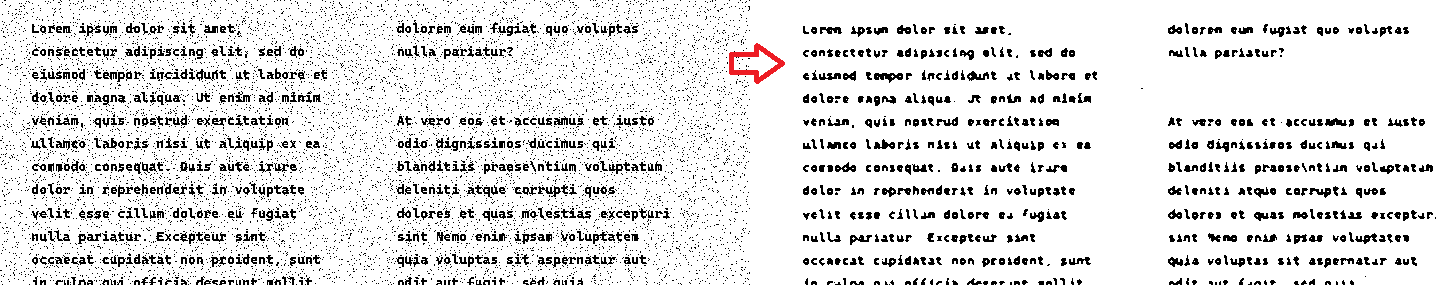
\includegraphics[scale=0.55]{./images/noise.png}
        \end{center}
  \legend{ \small Fonte: Autor.}
\end{figure}


\begin{figure}[htb]
        \caption{\label{horz} \small Resultado da aplicação de 2 iterações de dilatação com SE horizontal 5x5. }
        \begin{center}
            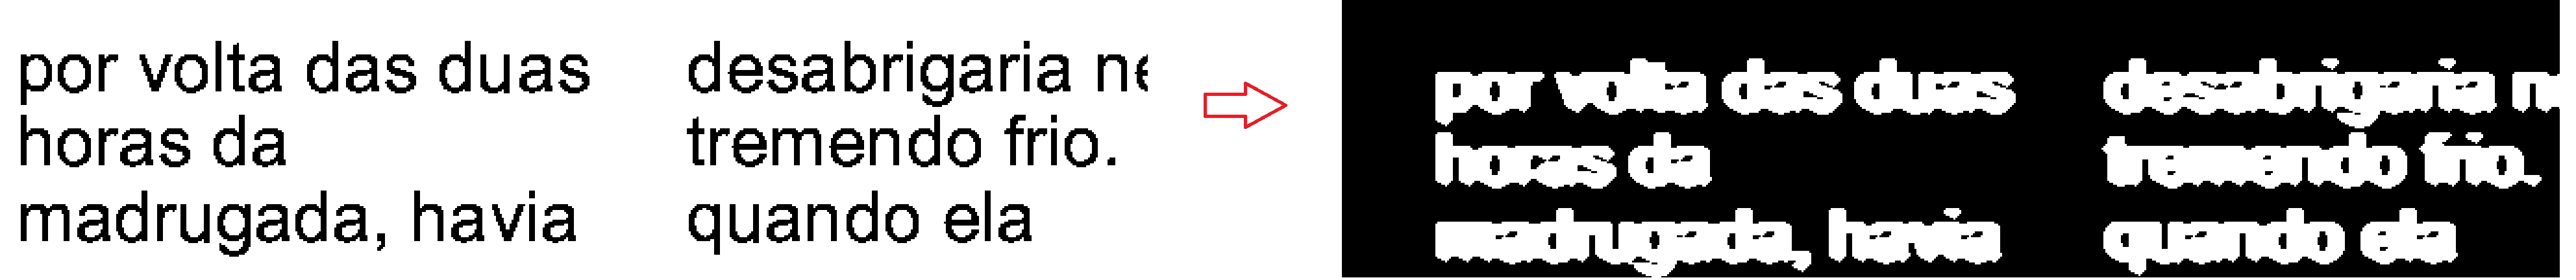
\includegraphics[scale=0.15]{./images/horizontal_5x5_aplicacao.png}
        \end{center}
  \legend{ \small Fonte: Autor.}
\end{figure}



\subsection{Componentes Conectados}

Podemos perceber que as operações de dilatação horizontal realmente melhoraram a conectividade entre caracteres adjacentes. Esses componentes conectados são as palavras individuais dentro da imagem. O conceito de componentes conectados é baseado em grafos, aplicável a imagens binárias, onde os pixels brancos representam os nós. Existem diferentes tipos de conectividade. Se considerarmos apenas os vizinhos de um pixel como à esquerda, à direita, acima e abaixo, temos o que chamamos de 4-conectividade \cite[2.5.2 Adjacency, Connectivity, Regions, and Boundaries]{gonzalez2008digital}. Ao adicionar as diagonais, temos a 8-conectividade.

O algoritmo apresentado no \autoref{cod-findcomp} é usado para encontrar esses componentes conectados e baseia-se em uma busca em profundidade, marcando os pixels visitados. A busca continua até não encontrar mais caminhos na imagem, considerando também as diagonais. Quando não há mais caminhos a serem explorados, o conjunto de pixels visitados forma um componente conectado. Este processo é repetido até que todos os componentes tenham sido identificados, atualizando os pontos mais à esquerda inferior e mais à direita superior do componente que é a \textit{bounding box} (retangulo) da palavra. Posteriomente, é desenhado um retangulo ao redor dessas palavras na imagem de saída. Opcionalmente, as palavras separadas podem ser escritas em uma nova imagem, visando a utilização posterior em tentativas de reconhecimento óptico de caracteres (OCR). 

Além disso, após a identificação dos componentes de texto, é realizada a filtragem para eliminar as \textit{bounding boxes} correspondentes à pontuação (virgulas, pontos) e manter apenas aquelas relacionadas às palavras. O \autoref{cod-group_bboxes} mostra como as palavras são então agrupadas em blocos com base em sua proximidade espacial. Para ilustrar  o processo de descoberta desses blocos, um vídeo é gerado para visualizar interativamente as etapas do algoritmo. 

\begin{codigo}[h]
  \caption{\small .}
 \label{cod-findcomp}
\begin{lstlisting}[language=python]
def find_connected_components_bboxes(image, min_area=0, connectivity=8):
    nbrs = [(1, 0), (-1, 0), (0, 1), (0, -1)]
    if connectivity == 8:
        nbrs.extend([(1, 1), (1, -1), (-1, 1), (-1, -1)])

    def dfs(y, x):
        nonlocal nbrs, image
        min_y, min_x, max_x, max_y = y, x, y, x
        stack = [(y, x)]
        while stack != list():
            cy, cx = stack.pop()
            if (
                0 <= cy < image.shape[0]
                and 0 <= cx < image.shape[1]
                and not visited[cy, cx]
                and image[cy, cx] == 255
            ):
                visited[cy, cx] = True
                min_y = min(min_y, cy)
                min_x = min(min_x, cx)
                max_x = max(max_x, cy)
                max_y = max(max_y, cx)

                for dy, dx in nbrs:
                    stack.append((cy + dy, cx + dx))
        return min_y, min_x, max_x, max_y

    visited = np.zeros(image.shape, dtype=bool)
    bounding_boxes = list()

    for y in range(image.shape[0]):
        for x in range(image.shape[1]):
            if not visited[y, x] and image[y, x] == 255:
                min_y, min_x, max_x, max_y = dfs(y, x)
                bounding_boxes.append((min_y, min_x, max_x, max_y))

    return bounding_boxes

\end{lstlisting}
\end{codigo}

\begin{codigo}[h]
  \caption{\small.}
 \label{cod-group_bboxes}
\begin{lstlisting}[language=python]
def group_bboxes(bboxes, max_distance, image) -> list[list]:
    """
    Group bboxes based on a max distance.
    `image` is video for purposes
    """
    result = list()
    rest_idxs = [i for i in range(len(bboxes))]
    while len(rest_idxs) > 0:
        close_idxs = [rest_idxs.pop()]
        bbox = bboxes[close_idxs[0]]
        counter = 0
        while counter < len(rest_idxs):
            r_idx = rest_idxs[counter]
            counter += 1
            dist = distance(bbox, bboxes[r_idx])
            if (dist < max_distance) or bbox_overlap(bbox, bboxes[r_idx]):
                close_idxs.append(r_idx)
                rest_idxs.remove(r_idx)
                bbox = enclosing_bbox([bbox, bboxes[r_idx]])
                counter = 0

                vid_img = image.copy()
                y, x, y2, x2 = bbox
                rectangle(vid_img, (y, x), (y2, x2), (0, 244, 55), 2)
                video_frames.append(vid_img)

        y, x, y2, x2 = bbox
        rectangle(image, (y, x), (y2, x2), (0, 244, 55), 2)
        result.append([bboxes[i] for i in close_idxs])
    return result
\end{lstlisting}
\end{codigo}

\subsection{Detecção e Reconhecimento de Caracteres}


O processo de reconhecimento de caracteres envolve três etapas principais: a detecção dos caracteres na imagem, a correspondência desses caracteres com os modelos predefinidos. O reconhecimento desses caracteres pode ser feito por correspondência de modelos (do inglês \textit{template matching}) \cite[12.2]{gonzalez2008digital}.  Durante o processo, as \textit{bounding boxes} são geradas para cada caractere detectado. O \autoref{cod-ocr} carrega modelos de letras predefinidos do diretório \texttt{./assets/letters/}. Os modelos são imagens binárias de letras individuais, como "v", "o", "l" e "t". Cada letra é invertida para garantir que os pixels de interesse (brancos) tenham o valor 255 e os pixels de fundo (pretos) tenham o valor 0. A imagem a ser comparada é a subimagem que contém o caractere que conseguimos detectar; em seguida, as \textit{bounding boxes} são ordenadas da esquerda para a direita, na ordem de leitura. Este recorte da letra é redimensionado para ter o mesmo tamanho das letras de referência. Para cada letra de referência, calculamos a similaridade entre a letra recortada e o modelo. A similaridade é medida contando o número de pixels brancos iguais nas duas imagens. A letra com a maior similaridade é considerada a melhor correspondência para a região.

\begin{codigo}[h]
  \caption{\small Função para reconhecimento de caracteres.}
 \label{cod-ocr}
\begin{lstlisting}[language=python]
# Pacote OCR
def string(img, letters):
    print(img.shape)
    orig = pim.convert_to_rgb(img)
    img = pim.invert(img)
    bbxs = pim.find_connected_components_bboxes(img, connectivity=8)
    # Start from leftmost
    bbxs = sorted(bbxs, key=lambda b: b[1])

    letter_sequence = []
    for b in bbxs:
        y, x, y2, x2 = b
        best_sim = 0
        best_letter = "-"
        for l, limg in letters.items():
            resized = pim.resize(img[y:y2, x:x2], *limg.shape)
            sim = 0
            for j in range(limg.shape[0]):
                for i in range(limg.shape[1]):
                    if resized[j, i] > 0:
                        if limg[j, i] > 0:
                            sim += 1
            if sim > best_sim:
                best_sim = sim
                best_letter = l
        letter_sequence.append(best_letter)

    return "".join(letter_sequence), orig
\end{lstlisting}
\end{codigo}





% Ao longo do processo, o algoritmo incorpora várias otimizações e ajustes de parâmetros para se adaptar a diferentes tipos de imagens de entrada e layouts de texto. Por exemplo, parâmetros como tamanho do kernel e contagens de iteração são ajustados dinamicamente com base nas características da imagem de entrada, como tamanho do texto e níveis de ruído.






\subsection{Operações Morfológicas}
\subsubsection{Dilatação}

 A dilatação morfológica é útil para preencher pequenos espaços entre objetos. No \autoref{udilate}, a função `understandable\_dilate` implementa a dilatação de forma "compreensível", mais compativel com a definição dada em \cite[9.2.2 Dilation]{gonzalez2008digital}.

 Nessa implementação a variável `kernel` representa o elemento estruturante, que define a forma e o tamanho da dilatação. Durante o processo, a imagem é percorrida pixel a pixel, e para cada pixel, verifica-se se pelo menos um dos pixels na vizinhança definida pelo kernel é branco (valor 255). Se pelo menos um dos pixels na vizinhança é branco, o pixel central é definido como branco (255) na imagem resultante. Caso contrário, o pixel central é definido como preto (0).

 Uma interepretação util é que o elemento estruturante define qual é a vizinhaça, onde tiver 1 no elemento indica que faz parte da vizinhaça, se tiver zero então não faz parte. Para cada x,y percorridos a imagem resultado é o máximo o valor de sua vizinhança definido pelo elemento estruturante.

\begin{codigo}[h]
  \caption{\small .}
 \label{udilate}
\begin{lstlisting}[language=python]
def understandable_dilate(image, kernel):
    result = np.zeros(image.shape)
    height = image.shape[0]
    width = image.shape[1]
    kernel_height = kernel.shape[1]
    kernel_width = kernel.shape[0]
    kernel_width_delta = kernel_width // 2
    kernel_height_delta = kernel_height // 2
    for y in range(height):
        for x in range(width):
            all_good = False
            for j in range(kernel_height):
                for i in range(kernel_width):
                    i_offset = i - kernel_width_delta
                    j_offset = j - kernel_height_delta
                    color = 0
                    if (
                        (x + i_offset) >= 0
                        and (x + i_offset) < width
                        and y + j_offset >= 0
                        and y + j_offset < height
                    ):
                        color = image[y + j_offset, x + i_offset]
                    kcolor = kernel[j, i]
                    if int(kcolor) * int(color):
                        all_good = True
                        break
                if all_good:
                    break
            if all_good:
                result[y, x] = 255
            else:
                result[y, x] = 0
    return result
\end{lstlisting}
\end{codigo}

  % Professora Bia, aqui eu disponho diferentes implementações de dilatação
  % understandable_dilate é o mais lento que tenta ser o mais entendivel possivel.
  % Ja fast_dilate2 é bem mais rapido, porém usa a função `maximum` da estrutura de dados matrix do  numpy.
  % é uma função que como o nome diz pega o maximo entre valores, mas funciona para matrix.
  % Eu dispus dessa maneira pra mostra que sei fazer todas as diferentes implementações,
  % mas pra ficar mais rapido e interativo é usado o fast_dilate2.
  % NOTE: Qualquer uma dessas implementações funciona para os propositos deste trabalho

No \autoref{fdilate2}, a função \texttt{fast\_dilate2} implementa uma dilatação morfológica mais rápida, aproveitando as operações de matriz do NumPy. A imagem é expandida com um preenchimento (\textit{padding}) adequado para evitar problemas de borda durante a aplicação (o elemento estruturante é chamado de kernel no código). Em seguida, o elemento estruturante é aplicado à imagem usando a função \texttt{np.maximum}, que calcula o máximo elemento a elemento entre a imagem resultante e o subconjunto da imagem com padding.

A imagem resultante começa com entradas zeradas e, à medida que iteramos sobre a altura $j$ e a largura $i$ do elemento estruturante, aplicamos essa função maximum em um subconjunto diferente da imagem com padding, dependendo de $j$ e $i$. Aplicamos isso apenas se o elemento estruturante for maior ou igual a 1 na altura $j$ e largura $i$. Isso efetivamente realiza uma dilatação, onde o pixel central de uma vizinhança é definido como o valor máximo dessa vizinhança. No entanto, observe que a vizinhança depende do elemento estruturante, apenas onde os valores são 1 são considerados vizinhança.

Ambas as implementações alcançam o mesmo resultado de dilatação morfológica, mas esta é mais eficiente devido ao uso de operações vetorizadas do NumPy. Isso resulta em uma execução mais rápida, especialmente em imagens grandes.

\begin{codigo}[h]
  \caption{\small.}
 \label{fdilate2}
\begin{lstlisting}[language=python]
def fast_dilate2(image, kernel):
    global counter 
    height, width = image.shape
    kernel_height, kernel_width = kernel.shape

    kernel_width_delta = kernel_width // 2
    kernel_height_delta = kernel_height // 2

    # We pad by the kernel delta, top, bottom, left and right
    padded_image = pad(
        image,
        kernel_height_delta,
        kernel_height_delta,
        kernel_width_delta,
        kernel_width_delta,
    )

    dilated = np.zeros(image.shape, dtype=np.uint8)
    for j in range(kernel_height):
        for i in range(kernel_width):
            if kernel[j, i] == 1:
                shifted_sub_image = padded_image[j : j + height, i : i + width]
                dilated = np.maximum(
                    dilated, shifted_sub_image
                )

    return dilated
\end{lstlisting}
\end{codigo}

\subsubsection{Erosão}

A erosão segue a mesma ideia da dilatação, mas com a operação sendo o \texttt{minimum} no lugar do \textit{maximum}. A iteração começa com a imagem resultante com todas as entradas 1 no lugar de 0. Na versão \texttt{understandable} da erosão, apenas quando \textbf{todos os pixels} da imagem se alinham com o elementento estruturante é que o pixel central é setado como 1 no lugar de \textbf{pelo menos um}. Vale ressaltar que a erosão não é necessária para o funcionamento do projeto, pois mesmo sem \texttt{closing} ou \texttt{opening}, que implicitamente usam erosão, o algoritmo é robusto para os casos de teste mencionados na introdução. A função \texttt{opening} é a operação de abertura, que consiste em primeiro realizar uma erosão seguida de uma dilatação. É útil para remover pequenos ruídos e separar objetos próximos, mas nesse trabalho, removemos esses ruídos pelo filtro da mediana.


\subsubsection{Contagens}
A contagem de linhas proposto baseia-se na análise de das bboxes que cercam as regiões de texto.
Primeiro verifica se a lista de caixas delimitadoras está vazia. As caixas são ordenadas verticalmente com base na coordenada y. Para cada caixa, calcula-se a sobreposição vertical com a caixa anterior. Se a sobreposição for menor que uma fração mínima, a caixa é contada como uma nova linha. A cada interação criamos uma imagem intermediaria para geração do video, nele exibimos as bboxes realçando corretamente as linhas de texto.

O algoritmo para contar colunas é similar ao de linhas, mas agora ordenamos pelo horizontal no lugar da vertical.
Mantemos uma variavel para contar o número de colunas e max\_right para acompanhar a coordenada x do canto inferior direito da caixa mais à direita encontrada até o momento.

Para cada caixa delimitadora ordenada, verifica-se se sua coordenada x do canto inferior esquerdo é maior do que a coordenada x do canto inferior direito da caixa mais à direita encontrada até o momento (max\_right). Se for, considera-se isso como o início de uma nova coluna e incrementa-se o contador de colunas (num\_columns). Também é desenhada uma linha vertical indicando o início da nova coluna na imagem de vídeo.

A coordenada x do canto inferior direito da caixa mais à direita (max\_right) é atualizada, se necessário.

No final, a imagem de vídeo atualizada é adicionada à lista video\_frames para visualização posterior, e o número total de colunas encontradas é retornado (num\_columns).


Para agrupar os paragrafos ou blocos A função começa inicializando uma lista vazia chamada result para armazenar os grupos de caixas delimitadoras agrupadas.

Em seguida, inicializa uma lista chamada rest\_idxs que contém os índices de todas as caixas delimitadoras não agrupadas inicialmente.

Enquanto ainda houver índices na lista rest\_idxs, o algoritmo continua a iterar:

Ele retira um índice da lista rest\_idxs e o adiciona à lista close\_idxs, que representa o grupo de caixas delimitadoras próximas.

Em seguida, calcula a distância entre a caixa delimitadora selecionada (bbox) e todas as outras caixas delimitadoras não agrupadas. Se a distância entre duas caixas delimitadoras for menor do que a max\_distance especificada ou se houver uma sobreposição significativa entre elas, as duas caixas são consideradas próximas o suficiente para serem agrupadas.

Se uma caixa delimitadora for adicionada ao grupo, ela é removida da lista rest\_idxs, e a função recalcula a caixa delimitadora que envolve todas as caixas no grupo atualizado.

Durante esse processo, a função também desenha retângulos em uma imagem de vídeo (representada por image) para visualização. Cada retângulo delimita o agrupamento de caixas delimitadoras.

Após a conclusão do processo de agrupamento para um determinado grupo de caixas delimitadoras próximas, o grupo resultante é adicionado à lista result.

Finalmente, a função retorna a lista result, que contém todos os grupos de caixas delimitadoras agrupadas com base na distância máxima especificada.




\chapter{Conclusão}

@@
Sumarização dos principais resultados e contribuições do trabalho.
Reflexão sobre o aprendizado durante o desenvolvimento do programa.
Sugestões para trabalhos futuros ou melhorias no programa.




\phantompart
\bibliography{Bibliografia}


%%%%%%%%%%%%%%%%%%%%%%%%%%%%%%%%%%%%%%%%%%%%%%%%%%%%%%
% ELEMENTOS PÓS-TEXTUAIS
%%%%%%%%%%%%%%%%%%%%%%%%%%%%%%%%%%%%%%%%%%%%%%%%%%%%%%


\postextual


\renewcommand{\chapnumfont}{\chaptitlefont}
\renewcommand{\afterchapternum}{}
% \include{Pos_Textual/Apendices}
% \include{Pos_Textual/Anexos}


\end{document}
